% This chapter should describe what was actually produced: the programs which were written, the hardware which was
% built or the theory which was developed. Any design strategies that looked ahead to the testing stage might 
% profitably be referred to (the professional approach again).

% Descriptions of programs may include fragments of high-level code but large chunks of code are usually best left % to appendices or omitted altogether. Analogous advice applies to circuit diagrams.
% Draw attention to the parts of the work which are not your own. Making effective use of powerful tools and 
% pre-existing code is often laudable, and will count to your credit if properly reported.
% It should not be necessary to give a day-by-day account of the progress of the work but major milestones may 
% sometimes be highlighted with advantage.

% ~4500 words

\documentclass[final,dissertation.tex]{subfiles}
\begin{document}

\chapter{Implementation (Due 6th April)}

In this chapter, I will describe how I implemented my project, describing challenges faced along the way. The implementation consists of the following:

\begin{itemize}
	\item A library for creating and processing Sphinx packets
	\item A library for sending and receiving messages on the Loopix network
	\item A command-line chat client that broadcasts messages to all clients on the network
	\item A testing framework for starting a test network
\end{itemize}

As Loopix uses the Sphinx packet format, I have implemented my own Java library of Sphinx. As such, the project is split into two libraries, with the low level cryptographic elements and packet format implemented in Sphinx, and the high-level network decisions such as path selection and routing implemented in Loopix. The Loopix library provides a basic event-driven API for sending and receiving messages.

\section{Sphinx Library}

The Sphinx library provides an API for creating and processing Sphinx packets as generated by the \verb|sphinxmix| Python package, and is based heavily on the package. This distinction is necessary to meet the project goal of binary compatibility with the existing Python Loopix implementation. \verb|sphinxmix|'s implementation deviates in several places when compared with the algorithm described in the Sphinx paper.

\subsection{Sphinx Parameters}

The \verb|SphinxParams| class encapsulates all of the cryptography and the various parameters for a Sphinx packet, such as the security parameter (key size), header size, body size, various hash functions, and the LIONESS wide block cipher.

As mentioned in section~\ref{sec:bouncy}, I used the BouncyCastle Java library for cryptographic primitives. 

These are: 
\begin{itemize}
\item AES-128-CTR
\item SHA-256
\item HMAC-SHA256
\end{itemize}

\subsection{Packet Creation}

Each Sphinx packet consists of two parts, the header and the body. The header contains information to correctly process the packet, and the body contains the encrypted payload. The packet has the following structure:

\begin{javacode}
public class SphinxPacket {
	public SphinxHeader header;
	public byte[] body;
}
\end{javacode}
	
\subsubsection{Sphinx Packet Header}

The header has the following structure:

\begin{javacode}
public class SphinxHeader {
	public ECPoint alpha;
	public byte[] beta;
	public byte[] gamma;
}
\end{javacode}

\begin{itemize}
	\item \verb|alpha| is an elliptic curve group element ($\alpha = g^b$) used to derive the per-hop shared secret required to authenticate and process the rest of \verb|SphinxHeader|. It is also used to decrypt a layer of the Sphinx body payload.
	\item \verb|beta| is a list of per-hop routing data and padding that is encrypted in a nested manner. Each layer contains routing commands that is defined and processed by a Sphinx node.
	\item \verb|gamma| is a HMAC-SHA256 message authentication code tag that covers \verb|alpha| and \verb|beta|
\end{itemize}

Header creation is handled in the \verb|SphinxClient| class. Header creation takes as input a sequence of mix nodes $\{n_0,..,n_{\nu-1}\}$ and their corresponding public keys $\{y_0,...,y_{\nu-1}\}$, and outputs a \verb|SphinxHeader| object and a list of per-hop shared secrets $\{s_0,...,s_{\nu-1}\}$. The function signature is given below.

\begin{javacode}
private static SphinxHeaderData createHeader(SphinxParams params,
	List<byte[]> path,
	List<ECPoint> keys,
	byte[] destination) throws CryptoException
\end{javacode}

Header creation first starts with the derivation of key material for each hop. This key material will be used to encrypt and authenticate the rest of the header, and the packet payload. Initially, a random $b \in_R \mathbb{Z}^*_q$ is chosen. This will be used as the initial blinding factor. A sequence of $\nu$ tuples $(\alpha_0, s_0, b_0),...,(\alpha_{\nu-1}, s_{\nu-1}, b_{\nu-1})$ is computed as follows:
\\
\begin{itemize}
	\setlength\itemsep{-0.4em}
	\item $\alpha_0 = g^b, s_0 = y_0^b, b_0 = h_b(s_0)*b$
	\item $\alpha_1 = g^{b_0}, s_1 = y_1^{b_0}, b_1 = h_b(s_1)*b_0$
	\item ...
\end{itemize}

\begin{itemize}
	\item $\alpha_n$ is the group element used in the Ephemeral Elliptic-curve Diffie-Hellman key exchange (ECDHE) to generate a shared secret. $\alpha_n$ can be thought of as an ephemeral public key. 
	%$\alpha_n$ is the exponentiation of the group generator $g$ with a blinding factor $b_{n-1}$. 
	
	\item $s_n$ is the shared secret for hop $n$. 
	%$s_n$ is the exponentiation of the hop's public key $x_n$ with the blinding factor $b_{n-1}$, that is $s_n = x^{b_{n-1}}_n$. 
	As the public key $y_n$ is of the form $g^{x_n}$, $s_n = (g^{x_n})^{b_{n-1}} = g^{{x_n}{b_{n-1}}}$. The shared secret is then passed into a key derivation function to produce an AES encryption key. The key derivation is done by passing the binary representation of the shared secret into the SHA-256 hash function and truncating the output to the security parameter $\kappa$.
	
	\item $b_n$, the blinding factor to be used for the next hop. This is computed by passing $s_n$ into a hash function $h_b$, which is implemented by using $s_n$ as an AES encryption key and encrypting a block of all zeroes. \footnote{The \verb|sphinxmix| package deviates from the paper here as the paper describes $b_n = h_b(\alpha_n, s_n)$, but the actual implementation ignores $\alpha_n$ and does $b_n = h_b(s_n)$.}
\end{itemize}


At the end of this derivation process, a list of $(\alpha_n, s_n, b_n)$ tuples, each corresponding to a hop in the path is generated. \verb|header.alpha| is set as $\alpha_0$.

The next step is to generate filler strings $\phi_i$ that serves as encrypted padding for $\beta$, routing information block. This is done by repeatedly encrypting the padding block with each hop's shared secret.

|possibly add phi diagram|

$\beta$ and $\gamma$ are generated next. Starting from the terminal hop, a sequence of headers $M_{\nu-1},M_{\nu-2},...,M_{0}$, where $M_i = (\alpha_i, \beta_i, \gamma_i)$ is computed as follows:

\begin{itemize}
	\setlength\itemsep{-0em}
	\item $\beta_{\nu-1} = \rho(h_\rho(s_{\nu-1}), \{{\text{destination-identifier}}\|\phi_{\nu-1}\})_{[0..\text{header size}]}$
	\item $\beta_{i} = \rho(h_\rho(s_{i}), \{n_{i+1} \| \gamma_{i+1} \| \beta_{i+1}\})_{[0..\text{header size}]}$ for $0 \le i < \nu - 1$
	\item $\gamma_i = \mu(h_\mu(s_{i}), \beta_i)$
\end{itemize}

\begin{itemize}
	\item $\rho$ is implemented using AES-128-CTR.
	\item $h_\rho$ is a hash function implemented using AES-128-CTR, by encrypting the string \verb|hrhohrhohrhohrho| using the parameter to $h_\rho$ as the encryption key.
	\item $\mu$ is implemented using HMAC-SHA256.
	\item $h_\mu$ is a hash function implemented using AES-128-CTR, by encrypting the string \verb|hmu:hmu:hmu:hmu:| using the parameter to $h_\mu$ as the encryption key.
	\item $\beta_i$ consists of either the destination identifier and the encrypted padding $\phi_{\nu-1}$, or a routing command $n_{i+1}$, a MAC $\gamma_{i+1}$ and a encrypted routing command block $\beta_{i+1}$ to forward to the next node.
\end{itemize}

\verb|header.gamma| is set to $\gamma_0$, and \verb|header.beta| is set to $\beta_0$. The final header structure when $\nu = 4$ is illustrated in Figure~\ref{fig:sphinx_header}. At the end of this process, a \verb|SphinxHeader| object with the necessary data $M_0$ and a list of per-hop shared secrets are created. The list of shared secrets will be later used for encrypting the payload.

|possibly add (beta, gamma) diagram|


\begin{figure}[h]
	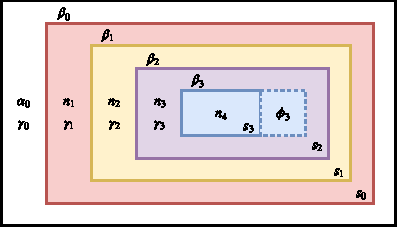
\includegraphics[width=\linewidth]{../figs/sphinx_header}
	\caption{Sphinx header for a packet with 4 hops}\label{fig:sphinx_header}
\end{figure}

\subsubsection{Sphinx Forward Packet Body}

Body creation is handled in the \verb|SphinxClient| class.  The function signature for creating an entire \verb|SphinxPacket| is given below.

\begin{javacode}
public static SphinxPacket createForwardMessage(SphinxParams params,
	List<byte[]> path,
	List<ECPoint> keys,
	Value destination,
	byte[] message) throws SphinxException
\end{javacode}

\verb|createForwardMessage| takes as inputs a sequence of mix nodes and their corresponding public keys as per the header generation section above, and a message $m$ of type \verb|byte[]|. It performs the following operations:

\begin{enumerate}
	\item \verb|message| is concatenated with the destination identifier and serialised using \verb|msgpack|, then padded to a fixed size.
	\item A call is made to \verb|createHeader| to generate a \verb|SphinxHeader| and the list of shared secrets $\{s_0,...,s_{\nu-1}\}$ to encrypt \verb|message| with.
	\item Starting from the terminal hop, \verb|message| is repeated encrypted using $\pi$ with a key derived from the hop's shared secret. That is,
		\begin{itemize}
			\setlength\itemsep{-0em}
			\item $\delta_{\nu-1} = \pi(h_\pi(s_{\nu-1}), m)$
			\item $\delta_i = \pi(h_\pi(s_{i}), \delta_{i+1})$
		\end{itemize}
	and as implemented:
	\begin{javacode}
byte[] delta = paddedBody;
for (int i = path.size() - 1; i >= 0; i--) {
	delta = params.pi(
		params.hpi(header.keys.get(i)), 
		delta
	);
}
	\end{javacode}
\end{enumerate}

The output of this process is the tuple $(M_0, \delta_0)$, which should be forwarded to the mix node $n_0$. The wire protocol for transmitting the tuple is determined by the consuming application. 

%\subsection{Packet Serialisation}
%
%msgpack, not actually used in Loopix

\subsection{Packet Processing}

\subsection{Challenges Faced}

Most of the challenges faced involves differences in language support for certain features between Java and Python.

There were a lot of byte array manipulations that primarily involved slicing arrays into different pieces, which is easily done in Python. However, in Java this caused the code to be very verbose and very hard to read.

The structure of how data is passed around also introduced readability issues, as the original implement made good use of tuple return types, which meant the creation of a lot of different classes in the Java codebase.

\section{Loopix Client Library}

\subsection{Public Key Infrastructure}

sqlite db

\subsection{Path Selection}

random selection, delay sampling

\section{Chat Client}

\section{Testing Framework}

\subsection{Unit Tests}

JUnit

\subsection{Continuous Integration}

Travis.CI (should this be under software engineering techniques in prep?)

\subsection{Docker Containers}

\section{Challenges Faced}

\end{document}